\section{Mathematical Model}\label{sec:mathmodel}
We assume as given a partially ordered ontology $O = (A, <)$ containing all relevant environmental artefacts for HAV. Initiatives towards identification of such an ontology are currently part of a number of R\&D projects on HAV, including the PEGASUS project\footnote{\url{www.pegasusproject.de}}. The ordering relation reflects the degree of precision of classification of objects, with $\bot$ (read: bottom) representing inconsistency, and $\top$ (read: top) denoting zero knowledge. The ontology contains different kinds of artefacts, e.g. relating to weather conditions (foggy, rain, snow, \ldots), road configurations (x-lane highway, T-type x lane intersection, \ldots), road conditions (dry, icy, aquaplaning, \ldots), roadside infrastructure (traffic signs, traffic lights, \ldots), traffic participants (car, truck, bicycle, pedestrian, animals, obstacles, \ldots), and surroundings of road segments (trees, buildings, \ldots). Objects in different categories are related by relations, and form separate sublattices, which are turned into a complete lattice by introducing a new top element. In this paper we will only refer to weather conditions, traffic situations, and traffic participants. Such ontologies are today in regular use as semantic basis for driving simulators such as SiLab. Sample ordering relations in the category of traffic participants are shown in Fig. \ref{fig1} below.
\begin{figure}
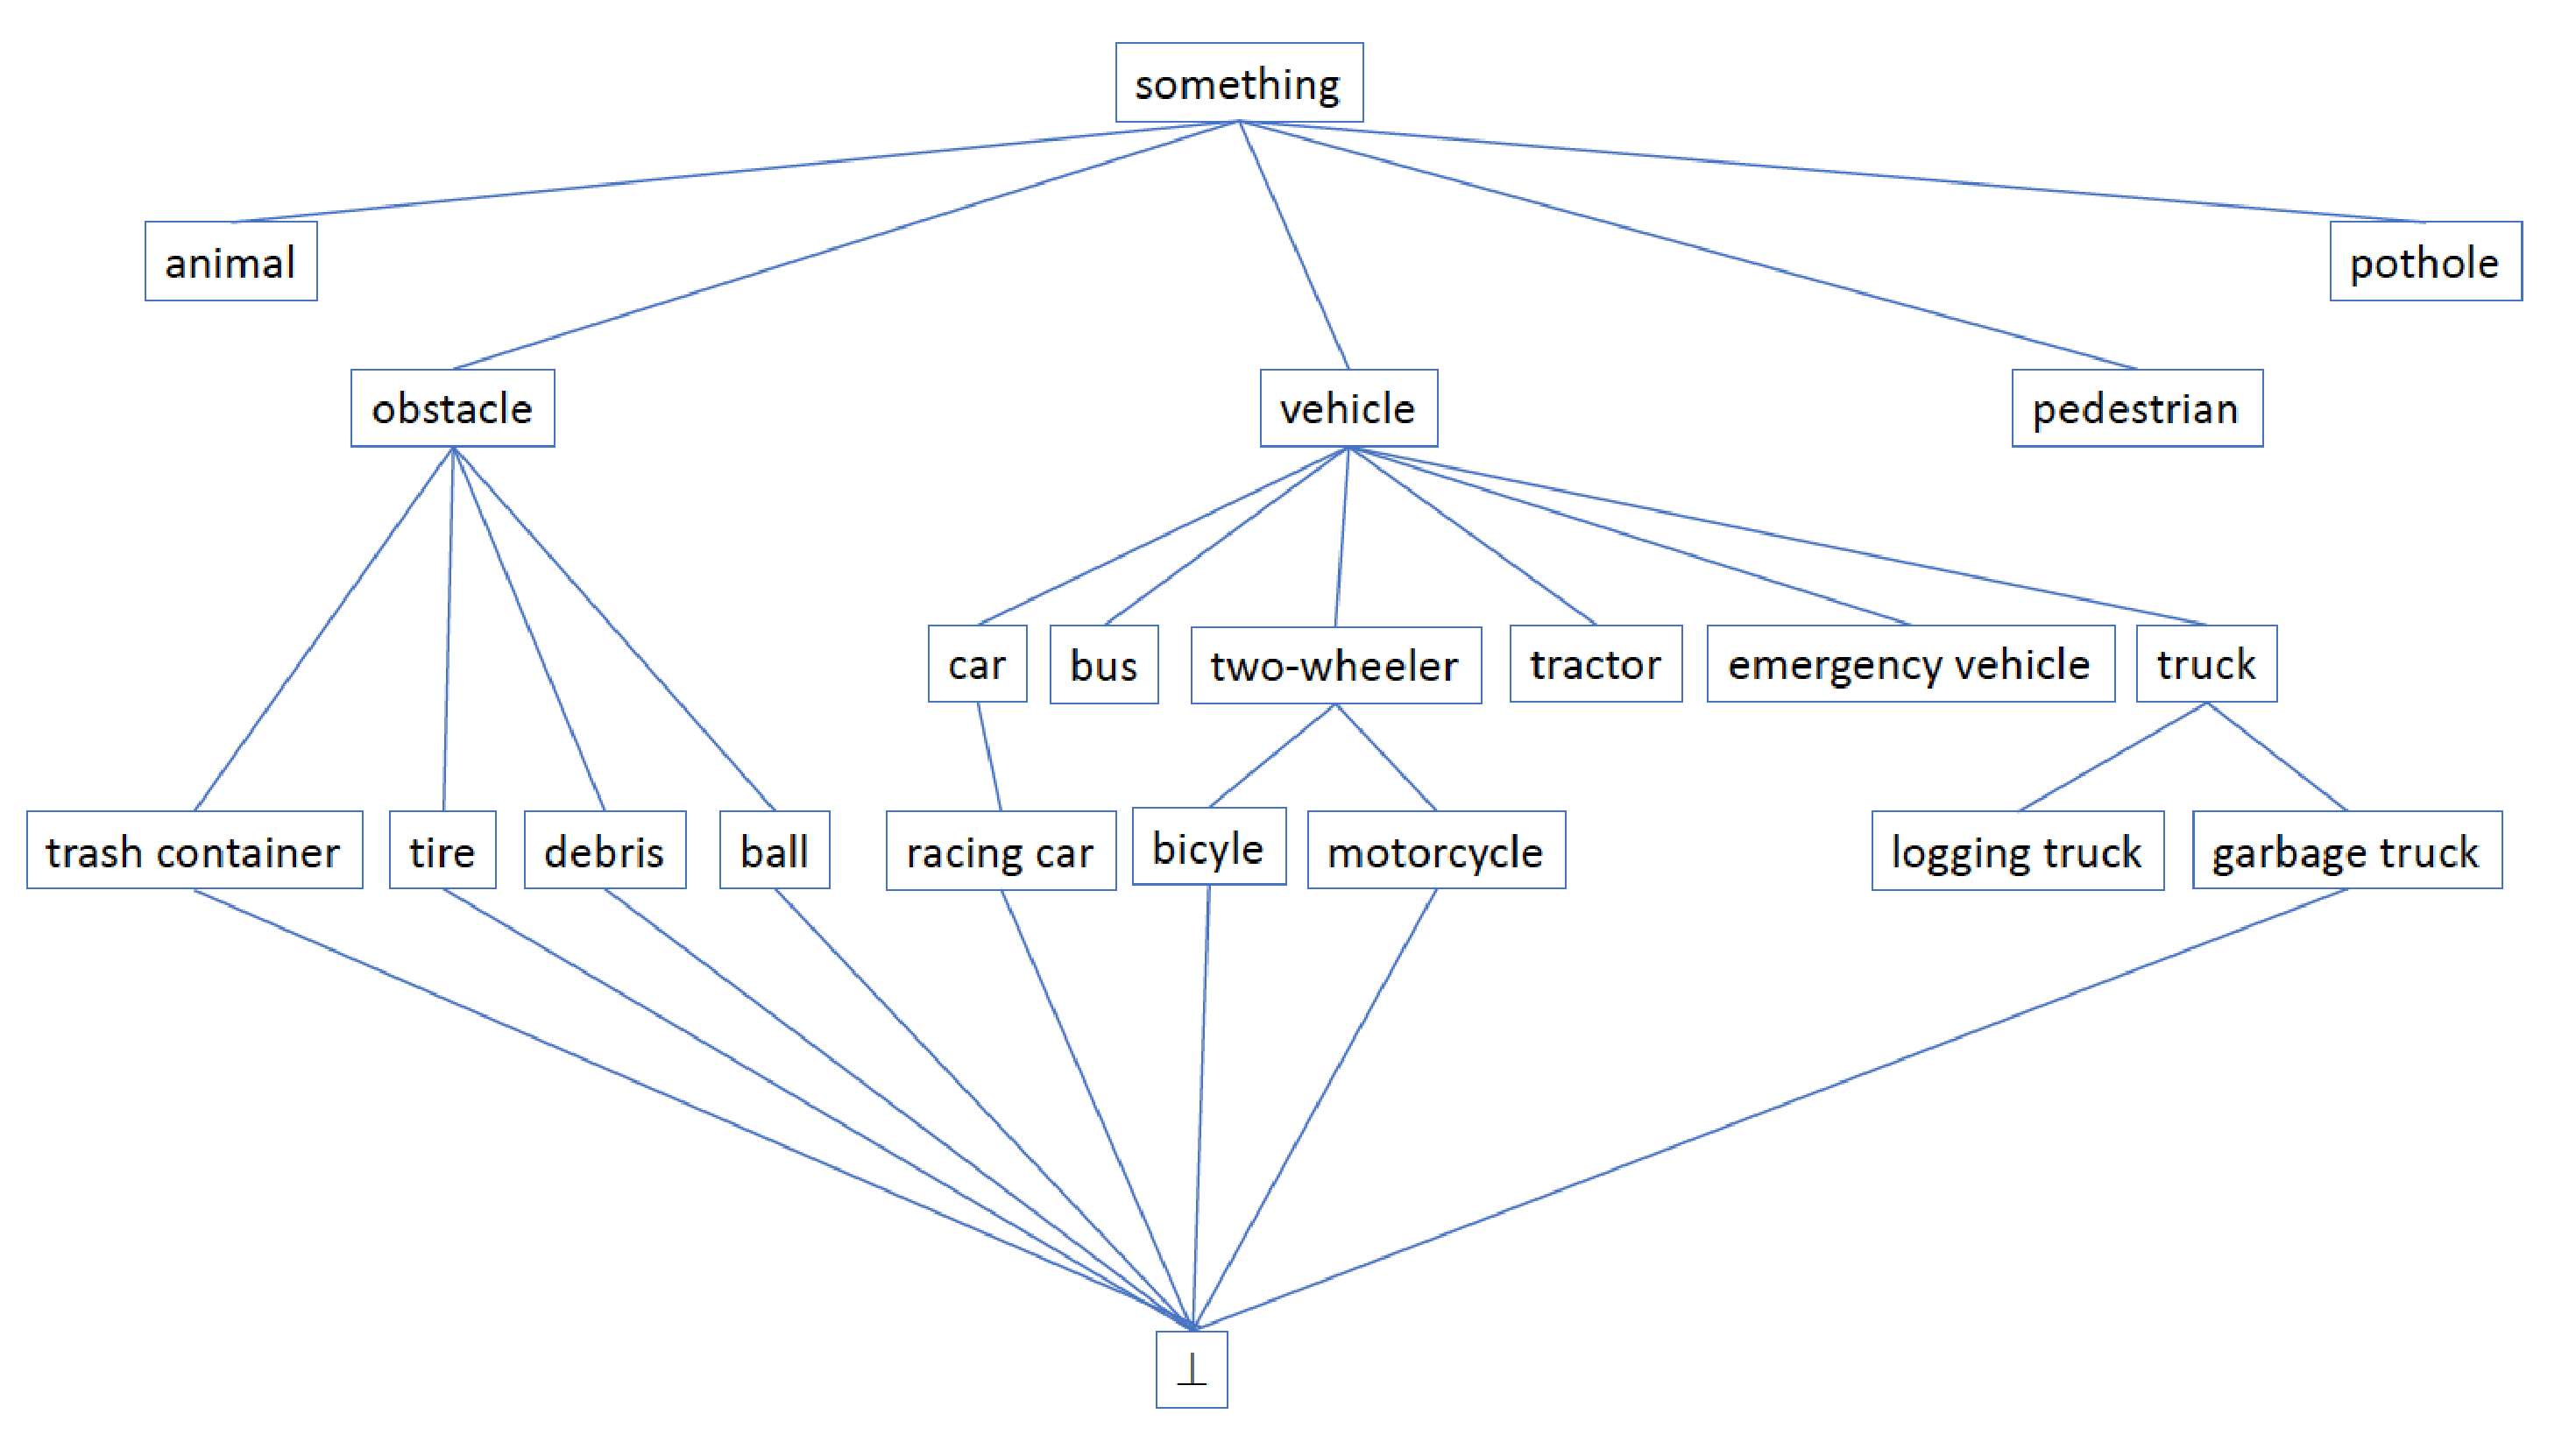
\includegraphics[width=\textwidth]{fig1.eps}
\caption{\textcolor{blue}{Sample ordering relations in the category of traffic participants}} \label{fig1}
\end{figure}

With each artefact  a  in the ontology, we assume as given a specification of its safety related aspects through a class definition cl(a). For artefacts of type road configurations, this includes specification of all geometric aspects including slope, number of lanes, width of lanes, etc. Road configurations are built from segments of a parametrized length. An operational design domain ODD is defined by constraints on types of road configurations, and constraints on prevailing weather conditions and road conditions. For each artefact veh of type vehicle, attributes of cl(veh) include the type of an instance of class road configuration, on which the vehicle is currently located, as well as its position, such as its longitudinal and lateral position on some lane of this instance of class road configuration. Moreover, each vehicle maintains its beliefs about its environment in appropriately typed attributes. Figure 2 below depicts the beliefs of ego driving on a country road: it believes the road surface is dry, that there is an obstacle in 250 m distance ahead blocking the lane, and that some vehicle of unknown type is approaching on the opposite lane. Importantly, cl(veh) contains as well a characterization of ODD-dependent dynamics of veh. We assume that these are given by probabilistic hybrid automata (cite \ldots), where mode changes are triggered based on believed changes of road configurations, weather conditions, road conditions, and observations of surrounding traffic and roadside infrastructure, and refer to this as pha(veh). A key point to be exploited is, that behavioral models are increasingly unconstrained along the generalization hierarchy: e.g., for class vehicle, the associated probabilistic hybrid automaton is constructed from those of the next level of specialization by introducing a new start state, branching non-deterministically into the entry states of the PHAs of cars, two-wheelers, trucks, emergency vehicles, etc. Similarly, we assume such models for pedestrians, animals, obstacles etc.

\begin{figure}
    \centering
    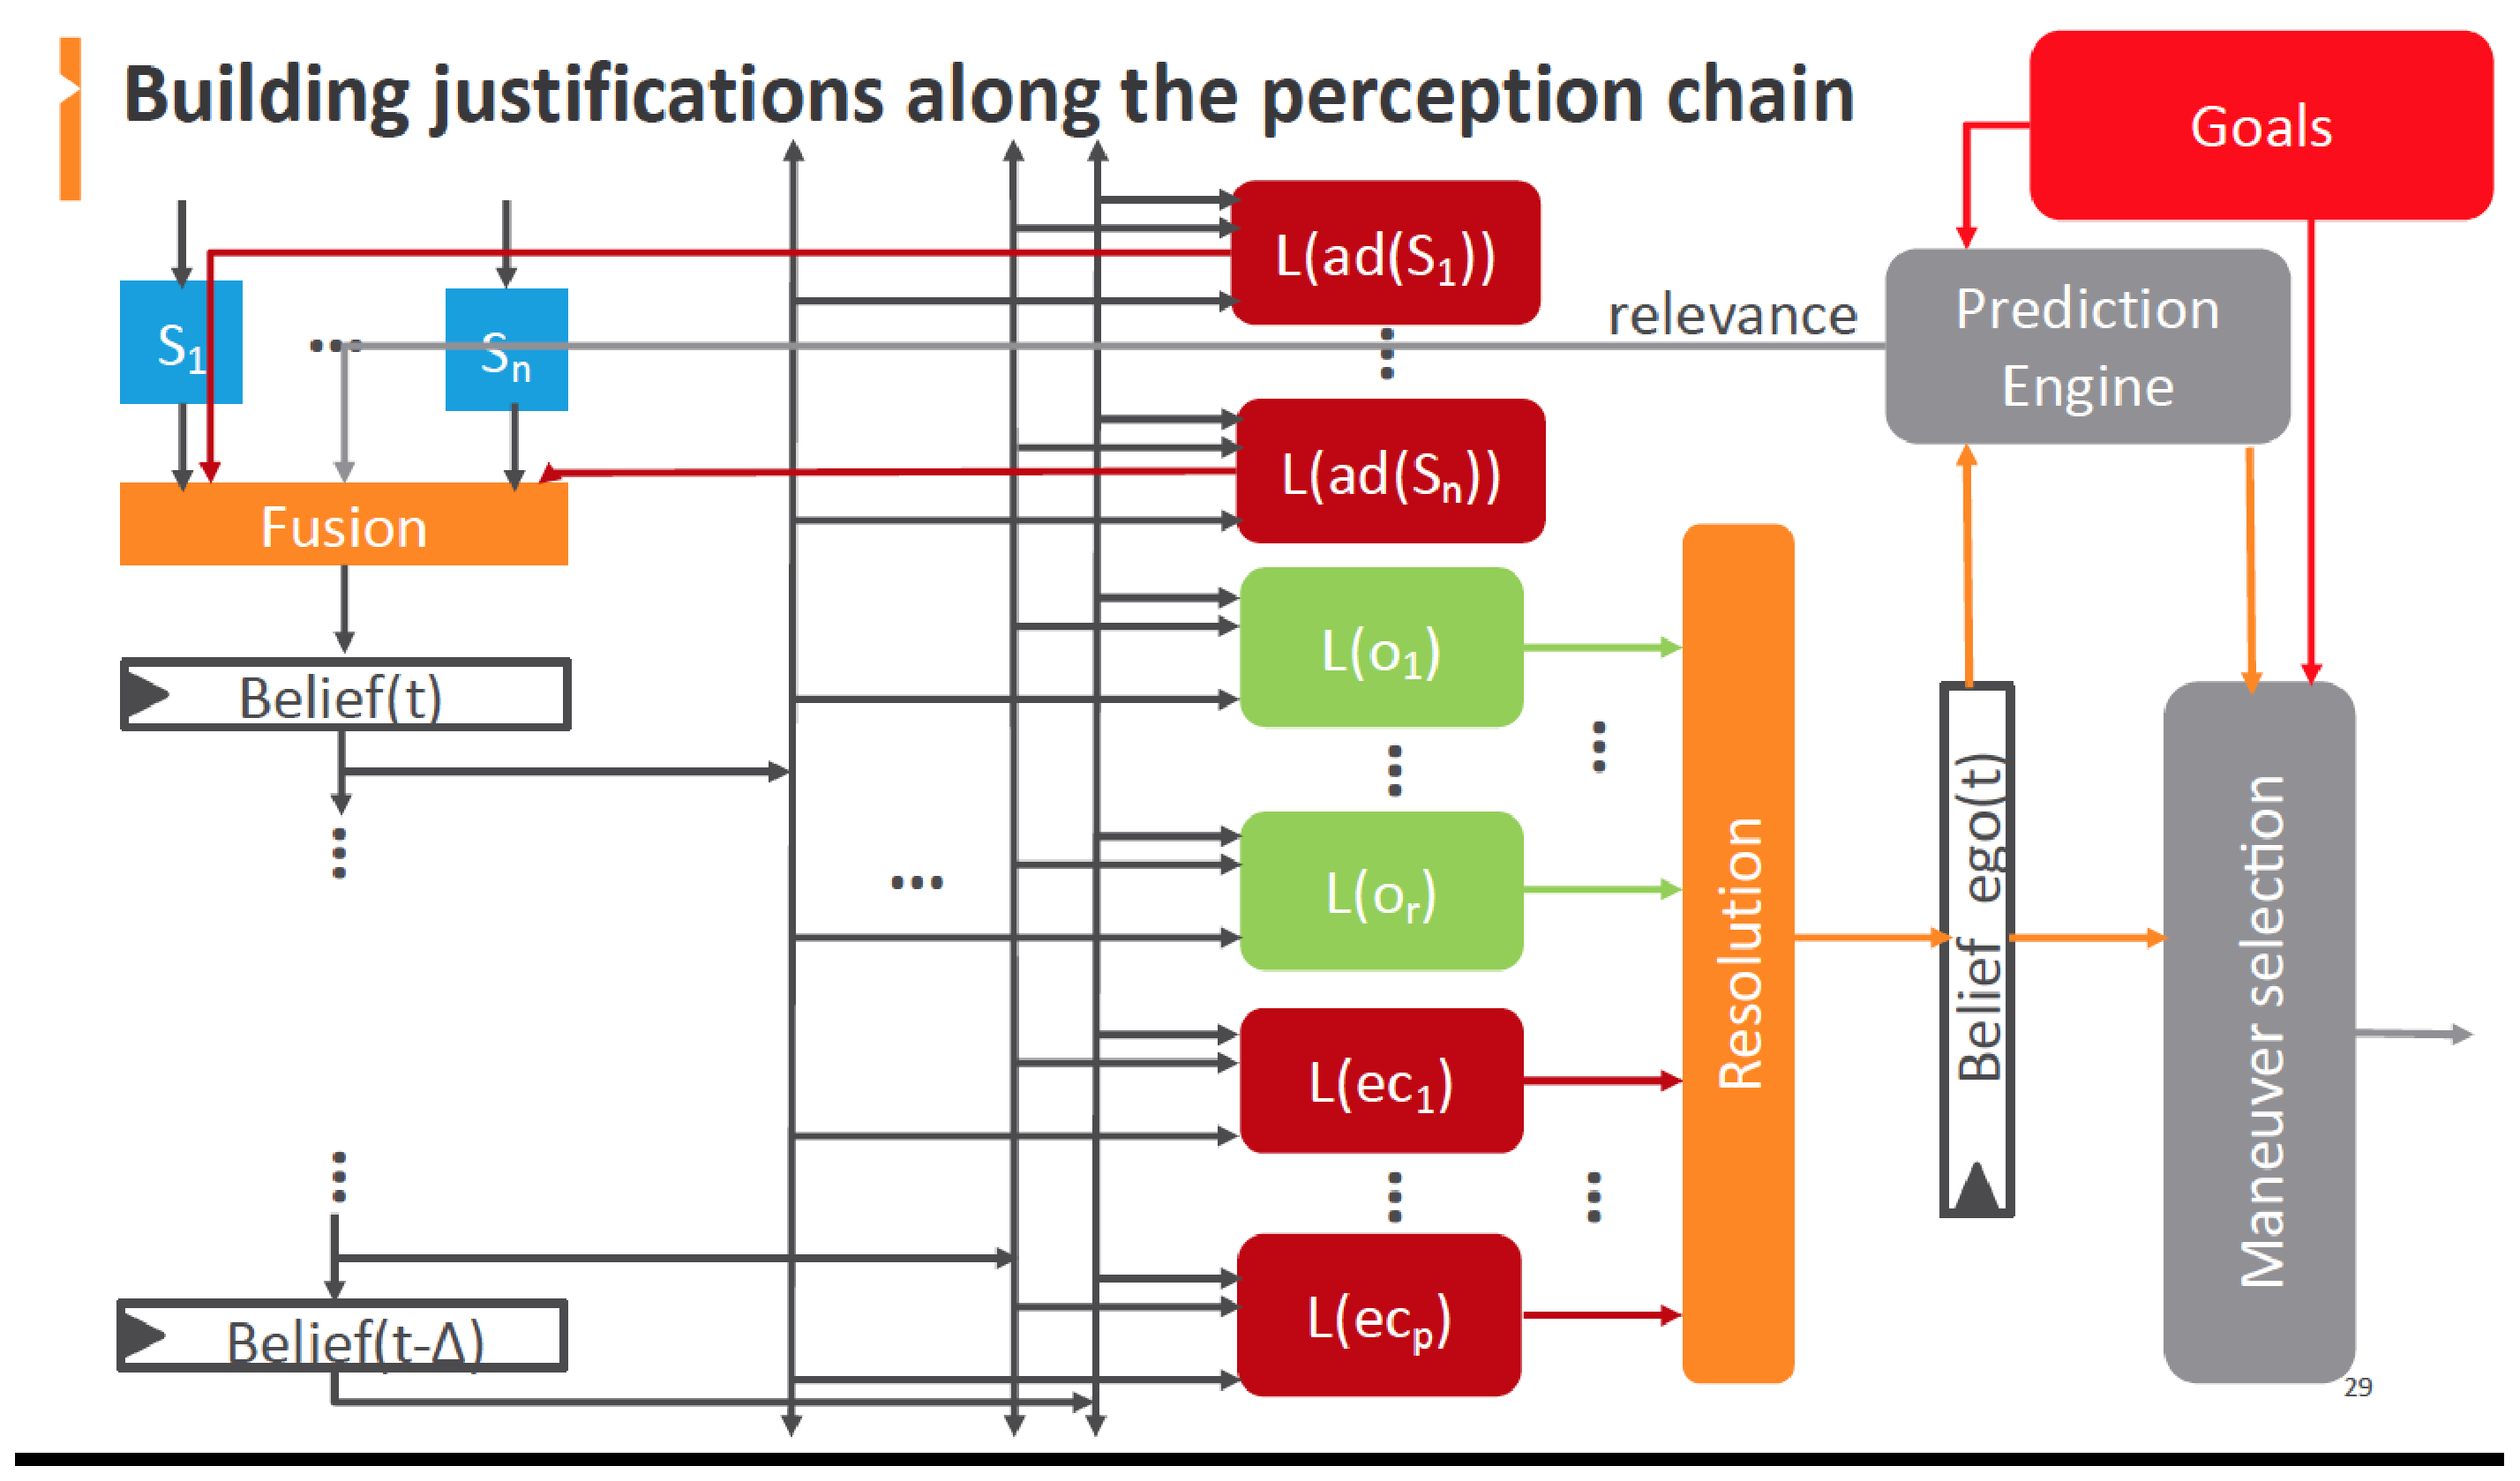
\includegraphics[width=\textwidth]{fig2.eps}
    \caption{\textcolor{blue}{Caption}}
    \label{fig2}
\end{figure}

Based on this, we can define a mathematical model of traffic evolution from the perspective of a given ego-vehicle. We define the electronic horizon of the ego vehicle to be the best-case range of perception of its on-board sensory system, and for simplicity of exposition in this paper assume this to be given by a rectangle aligned to the current pose of the ego vehicle centered at the geometric center of the ego vehicle. We call back- resp.\  front-horizon of ego the uttermost road segment still visible behind resp.\ in front of the car through its electronic horizon. The mathematical model is an infinite state transition system, whose state space is constructed as follows:
\begin{itemize}
\item It contains for each point in time t  all instances of road segments extending from the instance on which the ego car is currently positioned within its electronic horizon;
\item For each of the above road segments, it contains for time t  position and speed of all vehicles on the road segment, as well as road conditions and weather condition, positions of pedestrians, animals, obstacles, etc.
\end{itemize}
The (dense time) transition relation of the mathematical model is constructed as follows:
\begin{itemize}
\item New road segments are generated at the front- and lateral horizons by randomly instantiating new instance of class road segments while obeying the constraints of the ODD.\todo{MF: Warum relevant fuer eine Perzeptionskomponente im Einsatz, die ja auf einer konkreten Strasse unterwegs ist? Training ja...}
\item These new road segments are randomly attributed with road conditions and weather conditions observing consistency constraints and physical laws, and randomly filled with vehicles of randomly chosen type, with speeds and relative distances compliant to real observed traffic flow under the given ODD.
\item Where applicable, pedestrians are positioned randomly on newly generated road segments, observing traffic rules and dynamic models of pedestrians
\item Evolution of instances of objects of classes vehicles, pedestrian, animals follow the associated dynamic models
\item The evolution of the ego-vehicle follows the driving strategy determined from its beliefs about its environment as given by a probabilistic hybrid automaton.
\end{itemize}
We refrain for space reasons from giving the formal definitions, and refer to this transition system by \textit{TS(ego)} . A state of \textit{TS(ego)} is given by a valuation of all its observables. A run of \textit{TS(ego)} defines for each observable its evolution over time, thus including trajectories of all vehicles, pedestrians, animals, obstacles within ego's electronic horizon, including the evolution of the beliefs of the ego vehicle, and the evolution of its perceived road segments. We call \textit{RUNS(TS(ego)}) the set of all runs of \textit{TS(ego)}.

We can now formalize the meta requirement for the quality of the perception chain, up to the not yet formally defined notion of relevance, in a probabilistic linear time temporal logic, with observables defined by valuations of all attributes of all instances of classes within the electronic horizon of ego, over a typed first-order signature induced by the types of attributes in the ontology. Ideally, for each point in time, the ground truth of all relevant artefacts in ego's electronic horizon, in particular position and speed of surrounding traffic participants, road- and weather conditions, coincide exactly with ego's beliefs about these artefacts. We must relax this unachievable ideal first by considering standard measurement errors, and allowing classifications to be vague, as long as they are correct with respect to the ordering relation in the ontology, i.e.\ the ground truth classification is a specialization of the believed classification. Third, misclassifications and misperceptions will occur, but we want these to be bounded by the societally accepted level of risk. Assuming for each artefact $a$ a metric $d_a$ to measure the distance between ground truth and beliefs of $a$, and a safe level of measure tolerance $\delta_a$ we want almost always these to be consistent for a minimal time period $\Delta$ sufficient to take safe maneuver decisions for the HAV. This leads to the following formal requirement on the confidence of the perception chain of the HAV vehicle ego:

$\textit{Safe\_perception}(ego) = \forall a \in \textit{observables}(\textit{TS(ego)}):  \Box (\textit{relevant}(a) \Rightarrow$\hfil\\ $P(\Box_{\leq\Delta}d_a(a, \textit{belief}(a))> \delta_a) < r)$.

We will now propose methods to establish that \textit{TS(ego)} meets this overarching safety requirement. To this end, we will first introduce architectural constrains enabling such proofs, as expressed in the reference architecture of the perception chain elaborated in the next section.



